% PART I: RTX Project Description
%%%%%%%%%%%%%%%%%%%%%%%%%%%%
\chapter{Introduction}
%%%%%%%%%%%%%%%%%%%%%%%%%%%%

\section{Overview}
In this project, you will design a small real-time executive (RTX) and implement it on a Keil MCB1700 board populated with an NXP LPC1768 microcontroller . The executive will provide a basic multiprogramming environment, with five priority levels, preemption, simple memory management, message-based inter-process communication, a basic timing service, system console I/O and debugging support. 

Such an RTX is suitable for embedded computers which operate in real time. A cooperative, non-malicious software environment is assumed. The design of the RTX should allow its placement in ROM. 
Applications and non-kernel RTX processes must execute in the unprivileged level of LPC1768. The RTX kernel will execute in the privileged level
\footnote{We do not require application processes to use Process Stack Pointer (PSP). You may use the Main Stack Pointer (MSP) both for your kernel and non-kernel code. However non-trivial implementations that are not required such as using PSP for user processes and using memory protection unit to safe guard kernel sensitive data will be rewarded with bonus marks.}.
It has 32K of RAM for use by the RTX and application processes. It contains four timers, four UARTs and several other peripheral interface devices. The board has two RS-232 interfaces, from which UART0 is used for your RTX system console and UART1 is used for your RTX debug terminal.

\section{Summary of RTX Requirements}

The summary of the RTX requirements are listed as follows:

\begin{enumerate}
\item {\bf Scheduling Strategy}\\
      Four user priority levels plus an additional ``hidden" priority level for the Null process, preemption, no time slicing, FIFO (First In, First Out) discipline at each priority level.
\item {\bf RTX Primitives and Services}\\
      Refer to the Chapter \ref{p01_ch_rtx_api} (Description of RTX Primitives and Services).
\item {\bf RTX Footprint and Processor Loading} \\
      A reasonably {\em lean} implementation is expected. No standard C library function call is allowed in the kernel code.
\item {\bf Error Detection and Recovery}\\
      At minimum, the RTX kernel must detect one type of error: an attempt to \verb+send_message+ to or 
      \verb+set_process_priority+ of a non-existent process ID. The primitive will return an error code 
      (a non-zero integer value). No error recovery is required. 
      It may be assumed that the application processes can deal with this situation.
\end{enumerate}

%%%%%%%%%%%%%%%%%%%%%%%%%%%%%%%%%%%%%%%%%%%%%%%%%%%%%%%%%%%%%%%%%%%%%%%
\chapter{Description of RTX Primitives and Services}
%%%%%%%%%%%%%%%%%%%%%%%%%%%%%%%%%%%%%%%%%%%%%%%%%%%%%%%%%%%%%%%%%%%%%%%
\label{p01_ch_rtx_api}
This chapter lists the RTX primitive and services. You must implement theses as described and may not modify the prototypes in any way. The primitives listed below will always return a value, either a pointer or an \verb+int+ return code. In the latter case, the return code value of \verb+0+ indicates a success; non-zero value indicates a failure where applicable.

\section{The Application Programming Interface}
\label{sec_rtx_api}
The RTX user-space Application Programming Interface (API) is in \verb+rtx.h+. The \verb+rtx.h+ includes \verb+rtx_ext.h+ and \verb+commoh.h+ files. The \verb+rtx_ext.h+ is for students to put their self-defined RTX user API that is not required in this document. Note this is optional and you can leave this file empty if you do not implement not-required API. The \verb+common.h+ file contains macro definitions and data structures that both the kernel and the user-space code can include. The \verb+common.h+ includes \verb+common_ext.h+ file, which is for students to put self-defined macro definitions and data structures to be included by the kernel and the user-space code. Note that one can leave this file empty if no such extra macro definitions or data structures are needed. One {\em should not modify the contents of rtx.h and common.h}. A third-party testing software will include these two files. The \verb+rtx_ext.h+ and \verb+common_ext.h+ files can be freely modified.

\section{Memory Management}
\label{sec_memory}

The RTX supports a simple memory management scheme. The memory is divided into blocks of fixed size,
The size of each memory block is \verb+MEM_BLK_SIZE+ bytes and the number of these blocks is \verb+MEM_NUM_BLKS+, where both macros are defined in the \verb+common.h+ file.
The blocks can be used by the requesting processes for storing local variables or as envelopes for messages sent to other processes (see Section \ref{sec_ipc}). A block which is no longer needed must be returned to the RTX. \\

Two primitives are to be provided. \\ 
  \begin{itemize}
    \item[]{}
\begin{lstlisting}
void *request_memory_block();
\end{lstlisting}
    The \verb+request_memory_block+ primitive allocates a free memory block and returns a pointer to the memory block to the calling process. If no free memory block is available, the calling process is blocked until a free memory block becomes available. If several processes are waiting for a memory block and a block becomes available, the highest priority waiting process will get it. Within the same priority level, a first-come-first-served policy applies.\\ 
    \item[]{}
\begin{lstlisting}
int release_memory_block(void *memory_block);
\end{lstlisting}
      The \verb+release_memory_block+ primitive returns the memory block to the RTX. If there are processes waiting for a block, the block is given to the highest priority process, which is then unblocked. The caller of this primitive never blocks, but could be preempted (see Section \ref{sec_faq_sched}). Thus, it may affect the currently executing process.
\end{itemize}

\section{Processor Management}
\label{sec_processor}
One primitive is to be provided. \\
  \begin{itemize}[]
    \item[]{}
\begin{lstlisting}
int release_processor();
\end{lstlisting}
  \end{itemize} 
The \verb+release_processor+ primitive enables the process to relinquish the processor (the calling process voluntarily releases the processor). The calling process remains ready to execute and is put at the end of the ready queue of the same priority. The RTX will make new scheduling decision to determine the next process to run. Another process may possibly be selected for execution.

\section{Process Priority}
\label{sec_priority}
Process priorities have an integer priority value \verb+(0, 1, 2, 3, 4)+ where \verb+0+ is the highest priority level. Two primitives are to be provided to set and get the process priority. \\

  \begin{itemize}[]
    \item[]{}
\begin{lstlisting}
int set_process_priority(int process_id, int priority);
\end{lstlisting}
      The \verb+set_process_priority+ primitive sets the priority of the process with \verb+process_id+ to the value given in priority. A process may change priority of any process (including itself) except for i-processes (see Section \ref{sec_iprocs}). The priority of the null process may not be changed from level 4 and it is the only process that can be assigned to level 4 (see Section \ref{subsec_null_proc}). The caller of this primitive never blocks, but could be preempted. If the \verb+priority+ is higher than the priority of the current running process, and the process identified by \verb+process_id+ is ready to run, then the process identified by the \verb+process_id+ preempts the current running task. Otherwise, the current running process continues its execution. When the specified \verb+process_id+ does not exist or the \verb+priority+ is invalid, the function returns \verb+-1+. \\ 
    \item[]{}
\begin{lstlisting}
int get_process_priority(int process_id);
\end{lstlisting}
      This \verb+get_process_priority+ primitive returns the priority of the process identified by the \verb+process_id+ parameter. For an invalid \verb+process_id+, the primitive returns \verb+-1+.

  \end{itemize}
\section{Interprocess Communication}
\label{sec_ipc}
The RTX will support a message-based Interprocess Communication (IPC) discussed in lectures. Messages are carried in envelopes (memory blocks, see below) with a header which is less than \verb+64+ bytes. Two IPC primitives will be implemented. \\ 
  \begin{itemize}
    \item[]{}
\begin{lstlisting}
int send_message(int process_id, void *message_envelope);
\end{lstlisting}
The \verb+send_message+ primitive delivers to the destination process identified by \verb+process_id+ a message carried in a message envelope.
      The \verb+message_envelope+ argument is a pointer to the following general form structure:
\begin{lstlisting}
struct msgbuf {
#ifdef K_MSG_ENV
    void *mp_next;      /* ptr to the next message */
    int m_send_pid;     /* sender pid */
    int m_recv_pid;     /* receiver pid */
    int m_kdata[5];     /* extra 20B kernel data place holder */
#endif
    int  mtype;         /* user defined message type */
    char mtext[1];      /* body of the message */
};
\end{lstlisting}
      The fields that are enclosed in the \verb+#ifdef K_MSG_ENV+ and \verb+#endif+ form a data structure that kernel uses to manage the message passing. If the \verb+K_MSG_ENV+ is defined, then these fields will be exposed to user space. The user processes however should not access these fields even they are exposed to the user space. The kernel are responsible for modifying these fields. If the \verb+K_MSG_ENV+ is not defined, then the afore mentioned kernel fields will be hidden from the user space and the kernel is responsible to find space to store these fields.

      User processes are permitted to read and write the \verb+mtype+ and \verb+mtext+ fields. The \verb+mtype+ field takes a user defined message type. And the following macro defines the value of this field:
\begin{verbatim}
DEFAULT
\end{verbatim}
\begin{itemize}
\item[] A general purpose message.
\end{itemize}
\begin{verbatim}
KCD_REG
\end{verbatim}
\begin{itemize}
\item[] A message to register a command with the Keyboard Command Decoder Process (see Sectoin \ref{sec_kcd})
\end{itemize}
\begin{verbatim}
KCD_CMD
\end{verbatim}
\begin{itemize}
\item[] A message that contains a command to be handled by the receiving process (see Section \ref{sec_kcd}) .
\end{itemize}
\begin{verbatim}
CRT_DISPLAY
\end{verbatim}
\begin{itemize}
\item[] A message to display the message body to the RTX console (see Section \ref{sec_crt}).
\end{itemize}
\begin{verbatim}
KEY_IN
\end{verbatim}
\begin{itemize}
\item[] A message that contains an input key (may contain multiple characters if it is a control key) from keyboard (see Section \ref{subsec_io_procs}). 
\end{itemize}
These macros are defined in \verb+common.h+, which is included by \verb+rtx.h+ file as follows.
\begin{lstlisting}
#define DEFAULT     0
#define KCD_REG     1
#define KCD_CMD     2
#define CRT_DISPLAY 3
#define KEY_IN      4
\end{lstlisting}
You are free to add more user defined message type macros in the \verb+common_ext.h+ file.
Please note that both the host computer and the board are little-endian systems.

The \verb+mtext+ field is an array (or other structure) whose size is limited to 
the size of one memory block less 
%the message envelope header size and 
the total size of all other fields in the \verb+msgbuf+ structure.
The primitive changes the state of destination process to ready-to-execute if appropriate. The sending process is preempted if the receiving process was blocked waiting for a message and has higher priority, otherwise the sender continues executing. \\
% The header of the message will have the layout given in the course overheads. It also fills in the \verb+sender_process_id+ and \verb+destination_process_id+ fields in the message envelope. The fields \verb+sender_process_id+ and \verb+destination_process_id+ are both of type \verb+int+.
    \item[]{}
\begin{lstlisting}
void *receive_message(int *sender_id);
\end{lstlisting}
The \verb+receive_message+ is a blocking receive. If there is a message waiting, a pointer to the message envelope containing it will be returned to the caller. If there is no such message, the calling process blocks and another process is selected for execution. The sender of the message is identified through \verb+sender_id+, unless it is NULL. Note the \verb+sender_id+ is an output parameter and is not meant to filter which message to receive.

\end{itemize}

\section{Timing Services}
\label{sec_timing}

Unprivileged level processes obtain the timing service from RTX by the following primitive
\footnote{Unprivileged processes should not read kernel timer data directly. You are free to add a primitive to
return the kernel clock ticks to unprivileged processes should you find the delayed\_send primitive is not sufficient to provide the timing service you need. Self-defined user API can be added to the \texttt{rtx\_ext.h} file}. \\
\begin{itemize}[]
\item[]{}
\begin{lstlisting}
int delayed_send(int process_id, void *message_envelope, int delay);
\end{lstlisting}
The calling process does not block. The message (in the memory block pointed to by the second parameter) will be sent to the destination process (\verb+process_id+) after the expiration of the delay (timeout, given in {\em millisecond} units). 

\end{itemize}

\chapter{Required Processes}
\label{p01_ch_rtx_procs}
This chapter describes the processes which you must implement for the project. The initial priority of processes is in the range of \verb+{0, 1, 2, 3, 4}+ and is left as a free choice if it is not specified explicitly. The priority level 4 is a {\em hidden} priority level that is reserved for the Null process (see Section \ref{subsec_null_proc}. Note the I-processes (see Section \ref{sec_iprocs}) are not scheduled based on the priority. They are triggered by interrupts hence has no initial priority. 

\section{System Processes}
\label{sec_sys_procs}
System processes are those processes needed by the system to perform basic services (scheduling and I/O). You will need to make your design choice to determine which system processes require privileged level and which system processes may operate at unprivileged level.

\subsection{The Null Process}
\label{subsec_null_proc}

This process runs as the lowest priority process (level 4) in the RTX. The Null process is the only process assigned to level \verb+4+. Level \verb+4+ is basically a``hidden" priority level reserved for the Null process. This preserves the four levels of user priorities (levels \verb+0+, \verb+1+, \verb+2+ and \verb+3+). Process id \verb+0+ is reserved for the null process. Initially, the following pseudo code can be used to design your null process: \\
\begin{lstlisting}
loop forever
        release the processor
end loop
\end{lstlisting}
Once you have preemption working, then the ``\verb+release the processor+" line could be removed from the infinite loop.

\subsection{System Console I/O Processes}
\label{subsec_io_procs}

The system console is used for communication with the RTX and application processes. It consists of two devices: keyboard and CRT display. These two devices communicate serially with the microcomputer; using the receive and transmit lines of one of the two RS-232 ports. 

The RTX will include two system processes, the Keyboard Command Decoder (KCD) process and the CRT Display process. These processes work in cooperation with the UART interrupt handler i-process.

\subsubsection{The Keyboard Command Decoder (KCD) Process}
\label{sec_kcd}
A keyboard command starts with the prompt character \verb+%+, followed by a single letter command identifier and possibly additional command data. For example, \verb+%WS 12:45:00+ is a command that the wall clock process handles to start the wall clock display and setting the current time to \verb+12:45:00+ (where the command format is \verb+%WS hh:mm:ss+). The \verb+W+ is a single command identifier and the \verb+S 12:45:00+ following \verb+W+ are additional command data.

The keyboard command decoder (KCD) process is an unprivileged user-space process. 
It responds to two types of messages: command registration (\verb+KCD_REG+) and console keyboard input (\verb+KEY_IN+). The former contains the command identifier and the process id of the process to which such commands are to be delivered when entered on the console keyboard. The processing of messages received depends on their type:
\begin{itemize}
\item {Command Registration}\\
The command identifier is associated with the process id of the registrant. To register a command with KCD, a process will send a message with type of \verb+KCD_REG+ and the body of the message starts with \verb+%+ followed by the command identifier (for example \verb+W+ for wall clock related commands) and a null character to terminate the message (See Q3 in Section \ref{sec_ipc_faq} for a more detailed example).
KCD forwards any input command with a registered identifier to the corresponding registered process. Processes can register an already registered command identifier. KCD always forwards a command to the latest process that has registered the command's identifier.

\item {Keyboard Input}\\
  The UART i-process (see Section \ref{sec_iprocs}) forwards any key input to the KCD using the \verb+KEY_IN+ message. The KCD forwards this message to the CRT Display process to be echoed back to the console. KCD also queues the input keys inside its internal buffer. Upon receiving the ``enter'' key (i.e. \verb+\r+), KCD construct a single string using the queued characters inside the buffer. If the string starts with \verb+%+ followed by a registered command, then the KCD will forward the string to the corresponding registered process using a \verb+KCD_CMD+ message. The receiving process is responsible for handling the command. The message body contains the command string (including the \verb+%+ character and the ``enter'' key).

  If the command identifier is not registered, then KCD ignores the string and sends a message to the CRT display process to display ``Command not found''. If the string does not start with \verb+%+ or the length of the string exceeds the capacity of the message envelope, then KCD will ignore the string and send a message to CRT display process to display ``Invalid command''. 
  
  The relationship among the KCD process, CRT display process, UART I-Process and a process that has a command registered is illustrated in Figure \ref{fig_ipc_relationship}.

          \begin{minipage}{\linewidth}
            \centering
            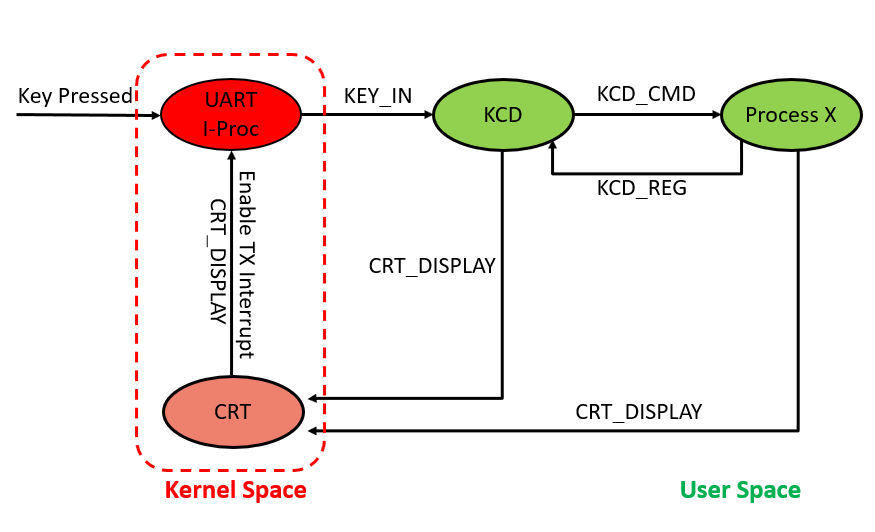
\includegraphics[width=5in]{figure/ipc/ipc_relationship}
            \captionof{figure}{System console I/O processes, uart i-process and a command handling process communication relationship.} 
            \label{fig_ipc_relationship}
          \end{minipage}
  
%The string input is sent to CRT display for output. If the string begins with a registered command identifier, it is also sent to the registered requester.
\end{itemize}

\subsubsection{The CRT Display Process}
\label{sec_crt}
The CRT display process is a privileged process. It responds to only one message type: a CRT display request. The message type is \verb+CRT_DISPLAY+. The message body contains the character string to be displayed to the RTX console. The string may contain control characters (e.g. newline and ANSI escape sequences et. al.). The string to be displayed is terminated by the null character.


% The process causes the string to be output to the console CRT.
In printing to the console display, the process works together the UART i-process. When the CRT display process needs to forward data to be displayed to the UART i-process, it reuses the message envelope it received which contains the \verb+CRT_DISPLAY+ type of message. It than triggers the UART transmission interrupt (See section \ref{sec_uart_programming}). Any message received but not forwarded to the UART i-process is freed using the \verb+release_memory_block+ primitive.

\section{Interrupt Processes (I-Processes)}
\label{sec_iprocs}
Two interrupt handling processes are required:

\subsection{The Timer I-Process}
\label{sec_timer_iproc}
The timer i-process is executed each time a hardware timer interrupt occurs. The timer i-process should handle the delivery of delayed send messages after the required time has expired.

\subsection{The UART I-Process}
\label{sec_uart_iproc}
The UART i-process uses interrupts for both the transmission and receiving of characters from the serial port (see Section \ref{sec_uart_programming}). No polling or busy waiting strategies may be implemented. The UART i-process forwards characters (or commands) received to the KCD by sending it the \verb+KEY_IN+ message, and also responds to messages received from the CRT display process (i.e. \verb+CRT_DISPLAY+ type message) to transmit characters to the serial port (see Figure \ref{fig_ipc_relationship}). The UART i-process turns off the transmit interrupt once it finishes transmitting the characters to the host machine serial port. The receiving interrupt is always on.  

\subsubsection{Three Hot Keys} 
The UART i-process is used to provide debugging services which will be used during the demonstration. Upon receiving a specific character (a hot key) as input, the UART i-process will print debugging information to the RTX system debug terminal, which is a polling terminal. The three required hot keys are:
\begin{itemize}
\item \verb+!+ hot key displays the processes currently on the ready queue(s) and their priority. 
\item \verb+@+ hot key displays the processes currently on the blocked on memory queue(s) and their priorities. 
\item \verb+#+ hot key displays the processes currently on the blocked on receive queue(s) and their priorities.
\end{itemize}
It is up to you whether you want to echo back the hot key input either to the debug terminal or the RTX console terminal. Not echoing it back to any terminal is an accepted solution. 

As well, you are free to implement other hot keys to help in debugging. For example, the \verb+$+ can be a hot key which lists the processes, their priorities, their states. The \verb+&+ can be yet another hot key which prints out the number of memory blocks available. Like all other debug prints, the hot key implementation should be wrapped in \\
\begin{lstlisting}
#ifdef _DEBUG_HOTKEYS
...
#endif
\end{lstlisting}
preprocessor statements and should be turned off during automated testing. If the automated test processes fail, you may be asked to turn the hot keys on again in determining why the test processes are failing.
Another hot key \verb+^+ may be used to display recent interprocess message passing. A (circular) log buffer keeps track of the 10 most recent \verb+send_message+ and \verb+receive_message+ invocations made by the processes; upon receiving a specific hot key, these most recent \verb+10+ sent and \verb+10+ received messages are printed to the debug console. The number \verb+10+ is used only as an example. The information printed could contain information such as:
\begin{itemize}
\item Sender process id 
\item Destination process id 
\item Message type 
\item First 16 bytes of the message text 
\item The time stamp of the transaction (using the RTX clock) 
\end{itemize}

\section{User Processes}
These processes operate at {\em unprivileged level} and will be used to demonstrate the operation of your system.

\subsection{User-Level Test Process}
\label{subsec_test_procs}

Write up to six user-space test processes to test your own OS. These test processes should run at unprivileged level and do not assume any kernel level data structures. These test processes only call the RTX user-space APIs (see Section \ref{sec_rtx_api}). The test processes should provide at least two and at most six test cases and finish testing within three minutes. The process id \verb+1+, \verb+2+, \verb+3+, \verb+4+, \verb+5+, and \verb+6+ are reserved for these processes.

Since the test processes have no knowledge of your detailed internal design, they only invoke the functions specified by the RTX user-space API. The test processes can use the timer that is not used by the RTX for timing testing.

We require the testing results to comply with the following format and you output the results to the debug UART terminal by polling (i.e. UART1):
\begin{verbatim}
Gid-TSN: START
Gid-TSN: some output
Gid-TSN: some output
Gid-TSN: x/M tests PASSED 
Gid-TSN: y/M tests FAILED
Gid-TSN: END
\end{verbatim}
In the above example output, the ``id'' is the Group ID. The ``N'' is the test suite ID, and ``M'' is the total number of testing cases. 
For example, assume that you are in group G99 and you have 3 testing cases in total in test suite 1, if two of the testing cases passed and one of the testing cases failed, the final testing results should be output to the putty terminal as follows:
\begin{verbatim}
G99-TS1: START
G99-TS1: some output 
G99-TS1: some output 
G99-TS1: some output 
G99-TS1: 2/3 tests PASSED
G99-TS1: 1/3 tests FAILED
G99-TS1: END
\end{verbatim}

\subsection{24 Hour Wall Clock Display Process}
\label{subsec_clock_proc}
This process registers itself with the Keyboard Command Decoder process as the handler for the \verb+%W+ command. 
\begin{itemize}
\item The \verb+%WR+ command will reset the current wall clock time to \verb+00:00:00+, starts the clock running and causes display of the current wall clock time on the console CRT. The display will be updated every second. 
\item The \verb+%WS hh:mm:ss+ command sets the current wall clock time to \verb+hh:mm:ss+, starts the clock running and causes display of the current wall clock time on the console CRT. The display will be updated every sec-ond. 
\item The \verb+%WT+ command will cause the wall clock display to be terminated. 
\end{itemize}

\subsection{Set Priority Command Process}
\label{subsec_priority_proc}
This process registers itself with the Keyboard Command Decoder process as the handler for the \verb+%C+ com¬mand. The \verb+%C+ command has two parameters: \\
\verb+%C process_id new_priority+ \\
The \verb+process_id+ and \verb+new_priority+ are integers. This command changes the priority of the specified process, \verb+process_id+, to \verb+new_priority+. The change in priority level is immediate. It could also affect the target process’s position on a ready queue or a blocked resource queue. The parameters must be verified to ensure a valid \verb+process_id+ and priority level are given. A \verb+%C+ command with illegal parameters will be ignored with an error message of ``Invalid command input'' printed on the console. 
\subsection{Stress Test Processes}
\label{subsec_abc_procs}
An important category of software tests are the stress tests. These tests seek to verify the behaviour of the system under heavy stress scenarios. One such scenario is depletion (or near depletion) of system resources. For the demonstration of this project, you will implement three processes whose behaviour is described below. The stress scenario being tested is depletion of memory blocks. \\ \\
Process A: 
\begin{lstlisting}
Register with KCD as handler of %Z command
loop forever
	p <- receive a message
	if the message(p) contains the %Z command then 
		release_memory_block(p)
		exit the loop
	else
		release_memory_block(p)
	endif
endloop
num = 0
loop forever
	p <- request memory block to be used as a message envelope
	set message_type field of p to “count_report”
	set message_text field of p to num 
	send the message(p) to process B
	num = num + 1
	release_processor()
endloop
/* note that Process A does not de-allocate any received envelopes in the second loop */
\end{lstlisting}
Process B:
\begin{lstlisting}
loop forever
	receive a message
	send the message to process C
endloop
\end{lstlisting}
Process C:
\begin{lstlisting}
perform any needed initialization and create a local message queue
loop forever
	if (local message queue is empty) then
		p <- receive a message
	else 
		p <- dequeue the first message from the local message queue
	endif
	if msg_type of p == “count_report” then
		if message_text field of p is evenly divisible by 20 then
			send "Process C" to CRT display using msg envelope p
			hibernate for 10 sec
		endif
	endif
	deallocate message envelope p
	release_processor()
endloop
\end{lstlisting}
The line ``\verb+hibernate for 10 sec+" is further expanded as:
\begin{lstlisting}	
q <- request_memory_block()
use q to delayed_send to itself with 10 sec delay and msg_type=wakeup10
loop forever
	p <- receive a message	//block and let other processes execute
	if (message_type of p ==  wakeup10) then
		exit this loop
	else 
		put message (p) on the local message queue for later processing
	endif
endloop
\end{lstlisting}
Notes:
\begin{itemize}
\item Process C has a local message queue (distinct from the incoming message queue maintained by the RTX) onto which it enqueues (in FIFO order) messages which arrive while it hibernates. It processes these mes-sages later.
\item For your own testing, set the priority levels for processes A, B and C to values which are most likely to cause memory block depletion in the RTX. During project demo, you may be asked to re-initialize your RTX with TA/instructor specified priorities for A, B, and C and vary the total number of message enve-lopes available.
%\item It is recommended that test processes A, B and C have process ids \verb+7+, \verb+8+, and \verb+9+ respectively. If you choose not to do this, you should have this information ready before the demonstration begins.

\section{Process ID Assignment}
To facilitate the project evaluation, we enforce the process ID assignment rule listed in Table \ref{tb_rtx_procs}. 
\begin{table}[h]
\begin{center}
\begin{tabular}{|l|l||l|l|}
\hline
process ID & Process & Process ID & Process \\ \hline \hline
0  & Null    & 8  &   B \\ \hline
1  & Test  1 & 9  &   C \\ \hline
2  & Test  2 & 10 & Set process priority process \\ \hline
3  & Test  3 & 11 & Wall clock display \\ \hline
4  & Test  4 & 12 & KCD \\ \hline
5  & Test  5 & 13 & CRT \\ \hline
6  & Test  6 & 14 & Timer i-process \\ \hline
7  & A       & 15 & UART i-process \\ \hline
\end{tabular}
\caption{Required RTX Processes}
\label{tb_rtx_procs}
\end{center}
\end{table}


\end{itemize}
\chapter{RTX Initialization}
\label{p01_ch_rtx_init}

To make the RTX more generally applicable, the RTX will be configured at initialization through the \verb+rtx_init+ system call.
%as specified in the RTX Configuration Table. This table has three sections:
The initialization contains three parts:
\begin{enumerate}
\item Memory configuration: memory block size, number of memory blocks created;
\item System process initialization: system process control blocks and stacks created; 
\item Application process initialization: user process control blocks and stacks created. 
\end{enumerate}

Chapter \ref{p01_ch_rtx_procs} (Required Processes) lists the processes to be created. Each entry contains the following data:
\begin{itemize} 
\item process id, 
\item priority, 
\item stack size, 
\item start address, and 
\item for system processes, whether the process is an i-process. 
\end{itemize}
{\em All initializations must take place after the RTX execution starts}.

\chapter{Deliverables and Demonstration}
\section{Deliverable}

% The project has three deliverables, where the first three deliverables are evaluated by in lab demonstrations.
The project has three deliverables, which will be evaluated through third-party automated testing grading software. 
The deliverables are as follows: 

\subsection{\bf RTX P1} 
This is the source code
% and documentation
of a tiny kernel which provides memory management, processor management and process priority services. You need to implement 
\begin{itemize}
\item APIs listed in Sections \ref{sec_memory}, \ref{sec_processor} and \ref{sec_priority}; 
\item processes in Sections \ref{subsec_null_proc} and \ref{subsec_test_procs}
      \footnote{Note you need to write the six user testing processes to demonstrate that your implementation meets the requirements.};  and 
\item the corresponding part in Chapter \ref{p01_ch_rtx_init}. 
\end{itemize}


\subsection{\bf RTX P2} 
This is the source code
% and documentation
of an RTX that builds on RTX P1. It added interprocess communications by message passing service and timing service.
\begin{itemize}
%\item make the kernel preemptive
%      \footnote{This involves some changes of existing code in P1 such as the release\_memory\_block() and
%      also the code of the null process.};
\item add APIs listed in Sections \ref{sec_ipc} and \ref{sec_timing};
\item finish implementing the timer i-process as described in Section  \ref{sec_timer_iproc}.
%     \ref{sec_sys_procs}, \ref{sec_iprocs} and \ref{subsec_clock_proc}; 
\item enhance user test processes in Section \ref{subsec_test_procs} so that they test this version of the kernel; and
\item implement the corresponding part in Chapter \ref{p01_ch_rtx_init}.     
 
\end{itemize}

\subsection{\bf RTX P3} 
This is the final RTX source code to implement the specifications
in Chapters \ref{p01_ch_rtx_api}, \ref{p01_ch_rtx_procs}, and \ref{p01_ch_rtx_init}
based on RTX P1 and RTX P2 implementations done previously. The main work is to provide console I/O services and perform stress testing of your final RTX.
To be more specific, you will implement the following items:
  \begin{itemize}
    \item the rest of system processes (KCD and CRT display processes) as described in Section \ref{sec_sys_procs} 
    \item the UART i-process as described in Section \ref{sec_uart_iproc}  
    \item the wall clock process as specified in \ref{subsec_clock_proc}
    \item the set process priority processes as specified in \ref{subsec_priority_proc}
    \item the three stress testing processes as specified in \ref{subsec_abc_procs} 
    \item the user test processes in Section \ref{subsec_test_procs} so that they test the final version of the kernel
    \item the corresponding part in Chapter \ref{p01_ch_rtx_init}.
  \end{itemize}
%It is possible that you will discover gaps or flaws in your original design during the implementation phase. You are allowed to adjust your implementation to reflect such discoveries. It is expected that you will document any major changes in the Final Project Report. 

\section{Demonstration}
The three milestones of the project are evaluated by demonstration.
%To make the re-grading fair, each group can only have one demo session per lab. If you still have questions after the demo session, then you may book lab office hours with the lab teaching team. However there will be no second demo. 

%\subsection{Demo Reservation and Cancellation}
%\begin{itemize}
%\item An on-line demo reservation link will be given to the class a couple of days before the demo. 
%\item You may cancel a demo reservation {\em 48 hours before} the reserved demo time slot by posting a private question on Piazza.
%\end{itemize}
\subsection{Demo Session Form Submission}
Before the first demo session, everyone in the group needs to sign the demo session form (available in LEARN Lab $\rightarrow$ Forms) and submit it to the demo form Dropbox on Learn. The agreement established in this form applies to all demo sessions. 

\subsection{The Demo Policy}
    \begin{itemize}
        \item The project is evaluated during the assigned demo time slot. It is recommended that you arrive the lab about 15 minutes earlier to set up your demo environment. The evaluation will end when the reserved demo time slot ends regardless whether you have finished demoing/answering all the items on the evaluation form or not. For the items that you are not able to finish during the reserved demo time slot, you will receive zero mark. 
        \item During the demo of your project, your original submitted RTX implementation archive file will be retrieved and the demo will use those files in the archive. No substitutions are allowed. It is student's responsibility to verify the submitted files are the correct version. We highly recommend to download your submission right after you submit it to confirm it is the correct version you want to submit.
        \item The demo is not some dry run to do additional debugging under "live" conditions. If minor bugs are discovered during the demo, depending on the complexity, you might be allowed to fix the bug, recompile and download and continue the demo with some penalty points deducted. Under no circumstances will file replacements be allowed during the demo. ``fixes" are basically limited to minor manual editing of a source file.
% Each demo for P1 and P2 is scheduled for a 30 minute slot maximum for in-person. The P3 demo slot is 55 minutes maximum.
If you want to fix minor bugs, the fix needs to be finished during the reserved demo time slot.
        \item You are only allowed to demo once. If you decide to go for the bonus demo
            \footnote{Bonus demo may not be available for some offerings},
            you are not allowed to do a regular demo again even you are unable to complete the bonus project demo. 
        \item ALL project group members are required to be presented during the demonstrations. 
    \end{itemize}
    
\subsection{The Demo Procedure}
\subsubsection*{P1 and P2 Demo Procedures} 
\begin{itemize}
\item {\bf Basic Functionality Demo}\\
You will need to demonstrate you have successfully completed the required APIs by using your own six test processes.
\item {\bf Source Code Spot Check} \\
An evaluator will ask each group member implementation questions.
%\item {\bf Contribution Check} \\
%Each group member will be asked what he/she has contributed to P1 implementation.
\end{itemize}

\subsubsection*{P3 Demo Procedure}
\label{subsec_p3demo}
\begin{itemize}
\item {\bf Basic Functionality Demo}\\
You will demonstrate the basic functionality of the RTX through commands line input. The evaluator will
\begin{itemize}
\item start, observe and stop wall clock display by using various \verb+%W+ commands;
\item check the hot keys output; and
\item set priority of processes by using \verb+%C+ commands.
\end{itemize}test of wall clock display 

\item{\bf Stress Test} \\
Your RTX will go through a stress testing demo by using processes A, B and C. The evaluator will
\begin{itemize}
\item reinitialize RTX with \verb+N+ (\verb+N=32+) envelopes, one combination of processes A,B and C priorities;
\item start test process activity by \verb+%Z+ command;
\item observe system operation (wall clock display as indicator), may also display trace buffer (is your have it implemented);
\end{itemize}
The above will be repeated with two other combinations of processes A,B and C priorities.
\item {\bf Contribution Check} \\
Each group member will be asked what he/she has contributed to the RTX (i.e. P1, P2 and P3) implementation.
\end{itemize}

%\subsection{Third Party Testing}
\section{Third-party Testing and Source Code File Organization}
\label{sec_ae}
    We will provide third party testing object code to replace the six testing processes written by students during the demo as part of the RTX functionality testing.
    %We will write third-party test cases to verify the correctness of your implementation.
    You will need to maintain the file organization of the project skeleton in the starter code.  
    There are dos and don'ts that you need to follow.
    \subsubsection*{Don'ts} 
      \begin{itemize}
        \item Do not move any file from the \verb+src+ directory to any other directories;
        \item Do not change the file names under the src directory;
        \item Do not make any changes of the contents of the \verb+rtx.h+ and \verb+common.h+ files;
        \item Do not change the existing function prototype in the given \verb+k_*.[ch]+ files; and
        \item Do not modify the \verb+ae.h+ files.
      \end{itemize}
    \subsubsection*{Dos}
      \begin{itemize}
        \item You are allowed to add new self-defined functions to \verb+k_*.[ch]+;
        \item You are also allowed to create new \verb+.h+ and \verb+.c+ files;
          \footnote{For example, you may want to create linked list data structure functions or some helper functions. You may want to create new files to hold these functions for better file organization.}.
        \item The newly created \verb+.h+ file is allowed to be included in the \verb+k_*.c+ file;
        \item Any new files you add to the project can be put into either the \verb+src+ directory or other directories you will create.
        %\begingroup \color{red}
        \item {You are allowed to make modifications of existing function contents in \verb+k_*.c+ as long as you keep the existing function prototype unchanged.}
        \item {You are allowed to make modifications of existing function contents in \verb+ae.c+ as long as you keep the existing function prototype unchanged.}
        %\endgroup
      \end{itemize}

  Note that the \verb+main_svc.c+ calls third-party testing by calling \verb+ae_init+ function which the third-party testing software implements. The function prototypes of this function does not change. But the implementation of this function may change in real testing.
Do not delete the lines in the \verb+main_svc.c+ where this function is invoked.
During the third-party testing, the files with prefix of \verb+ae_+ will be replaced by more complicated testing cases than the ones published on GitHub. 

%%% Local Variables:
%%% mode: latex
%%% TeX-master: "main_book"
%%% End:
